% % % % % % % % % % Document class % % % % % % % % % %
\documentclass[pdflatex, sn-apa]{sn-jnl}

% % % % % % % % % % Packages % % % % % % % % % %
\usepackage{algorithm}
\usepackage{algorithmic}
\usepackage{amsfonts}
\usepackage{amsmath}
\usepackage{amssymb}
\usepackage{amsthm}
\usepackage{anyfontsize}
\usepackage[title]{appendix}
\usepackage[utf8]{inputenc}
\usepackage[style = apa, backend = biber]{biblatex}
\usepackage{booktabs}
\usepackage{tabu}
\usepackage{arydshln}
\usepackage[inline]{enumitem}
\usepackage[T1]{fontenc}
\usepackage{graphicx}
\usepackage{latexcolors}
\usepackage{listings}
\usepackage{lmodern}
\usepackage{manyfoot}
\usepackage{mathrsfs}
\usepackage{microtype}
\usepackage{multirow}
\usepackage{nicefrac}
\usepackage{orcidlink}
\usepackage{textcomp}
\usepackage{xcolor}
\usepackage{tikz}
\usetikzlibrary{arrows.meta, matrix, positioning, shapes}

% % % % % % % % % % Commands % % % % % % % % % %
\addbibresource{bibliography.bib}

\renewcommand{\arraystretch}{1.15}

\newcommand{\I}{\mathcal{I}}
\newcommand{\B}{\mathcal{B}}
\newcommand{\D}{\mathcal{D}}
\newcommand{\X}{\mathcal{X}}

\definecolor{uclm}{HTML}{B60034}

% % % % % % % % % % Styles % % % % % % % % % %

% Node style
\tikzset
{
    every node/.style =
    {
        align = center
    }
}

% Path style
\tikzset
{
    every path/.style =
    {
        -stealth,
        draw,
    }
}

% Function style
\tikzset
{
    function/.style = 
    {
        rectangle,
        minimum size = 0.75cm,
        font = \footnotesize,
        align = center,
        fill = seagreen,
        draw = white,
        text = white,
        line width = 0cm
    }
}

% Dataset style
\tikzset
{
    dataset/.style = 
    {
        cylinder,
        minimum size = 2cm,
        font = \footnotesize,
        shape border rotate = 90,
        shape aspect = 0.4,
        align = center,
        fill = steelblue,
        draw = white,
        text = white,
        line width = 0cm
    }
}

% Algorithm style
\tikzset
{
    algorithm/.style =
    {
        diamond,
        minimum size = 0.75cm,
        font = \footnotesize,
        align = center,
        fill = uclm,
        draw = white,
        text = white,
        line width = 0cm
    }
}

% Preference matrix style
\tikzset
{
    preference/.style =
    {
        cylinder,
        minimum width = 1.75cm,
        minimum height = 1.5cm,
        font = \footnotesize,
        shape border rotate = 90,
        shape aspect = 0.25,
        align = center,
        fill = steelblue,
        draw = white,
        text = white,
        line width = 0cm
    }
}

% Instance style
\tikzset
{
    instance/.style = 
    {
        cylinder,
        minimum width = 1.5cm,
        minimum height = 1cm,
        font = \footnotesize,
        shape border rotate = 90,
        shape aspect = 0.25,
        align = center,
        fill = steelblue,
        draw = white,
        text = white,
        line width = 0cm
    }
}

% Prediction style
\tikzset
{
    prediction/.style =
    {
        circle,
        minimum size = 0.75cm,
        font = \footnotesize,
        fill = chromeyellow,
        draw = white,
        text = white,
        line width = 0cm
    }
}

% Annotation style
\tikzset
{
    annotation/.style =
    {
        align = center,
        font = \footnotesize
    }
}

% % % % % % % % % % Document % % % % % % % % % %
\begin{document}

% % % % % % % % % % Title % % % % % % % % % %
\title{A comparative analysis of rank aggregation methods for the partial label ranking problem}

\author*[1,2]{\orcidlink{0009-0001-5701-7351} \fnm{Jiayi} \sur{Wang}}\email{Jiayi.Wang@campus.lmu.de}

\author[3,4]{\orcidlink{0000-0003-1777-8540} \fnm{Juan C.} \sur{Alfaro}}\email{JuanCarlos.Alfaro@uclm.es}

\author[1,2]{\orcidlink{0000-0001-6988-6186} \fnm{Viktor} \sur{Bengs}}\email{Viktor.Bengs@ifi.lmu.de}

\affil[1]{\orgdiv{Chair of Artificial Intelligence and Machine Learning}, \orgname{Ludwig-Maximilians-Universität München}, \orgaddress{\city{Munich}, \postcode{80799}, \country{Germany}}}

\affil[2]{\orgdiv{Munich Center for Machine Learning}, \orgaddress{\city{Munich}, \country{Germany}}}

\affil[3]{\orgdiv{Departamento de Tecnologías y Sistemas de la Información}, \orgname{Universidad de Castilla-La Mancha}, \orgaddress{\city{Ciudad Real}, \postcode{13071}, \country{Spain}}}

\affil[4]{\orgdiv{Laboratorio de Sistemas Inteligentes y Minería de Datos}, \orgname{Universidad de Castilla-La Mancha}, \orgaddress{\city{Albacete}, \postcode{02071}, \country{Spain}}}

% % % % % % % % % % Abstract % % % % % % % % % %
\abstract
{%
    The \textit{label ranking} problem is a supervised learning scenario in which the learner predicts a \textit{total order} of the class labels for a given input instance. 
    %
    Recently, research has increasingly focused on the \textit{partial label ranking} problem, a generalization of the label ranking problem that allows \textit{ties} in the predicted orders.
    %
    So far, most existing learning approaches for the partial label ranking problem rely on approximation algorithms for rank aggregation in the final prediction step.
    %
    This paper explores several alternative aggregation methods for this critical step, including scoring-based and probabilistic-based rank aggregation approaches.
    %
    To enhance their suitability for the more general partial label ranking problem, the investigated methods are extended to increase the likelihood of producing ties.
    %
    Experimental evaluations on standard benchmarks demonstrate that scoring-based variants consistently outperform the current state-of-the-art method in handling incomplete information. In contrast, probabilistic-based variants fail to achieve competitive performance.
}

% % % % % % % % % % Keywords % % % % % % % % % %
\keywords
{%
    Preference learning, %
    Optimal bucket order problem,  %
    Rank aggregation problem, %
    Label ranking problem, %
    Partial label ranking problem
}

\maketitle

% % % % % % % % % % Introduction % % % % % % % % % %
\section{Introduction}\label{section:introduction}

The rapid proliferation of \textit{large language models} has significantly heightened interest in \textit{preference learning}.
%
This field explores preference information in various forms, including \textit{absolute} nature such as utility scores, binary, or ordinal data, as well as \textit{relative} nature like total orders, top-k lists, or partial orders.
%
This attentiveness arises from the significant contributions of preference learning techniques to optimizing the fine-tuning process of large language models, as discussed in recent surveys on the subject by \textcite{kaufmann_survey_2024}. 
%
This renewed interest encompasses a broad range of topics, from fundamental areas such as \textit{statistical preference models} \parencite{firth_davidson-luce_2019, henderson_modelling_2024} to advanced domains like \textit{preference-based bandits} \parencite{bengs_preference-based_2021} or \textit{preference-based reinforcement learning} \parencite{wirth_survey_2017}.
%
%

Another important area within this range is \textit{label ranking}, which focuses on the instance-dependent prediction of \textit{total orders} over a set of predefined class labels \parencite{hullermeier_label_2008}.
%
For example, consider predicting the order of movies (class labels) based on their popularity for a specific user (instance). 
%
The learner's objective is to learn a mapping from the user's features to a total order over the available movies, ensuring alignment with the user's preferences.
%
%

Although there is extensive literature on this learning problem, its applicability to real-world scenarios remains limited. 
%
For example, when predicting movie popularity, label ranking methods inherently produce a total ordering of movies.
%
However, it is questionable whether every user can consistently classify each pair of movies as being either more or less preferred.
%
This limitation is not restricted to typical recommendation system domains like movies or music; it also arises in broader scenarios involving human preferences.
%
A notable example is the preferences among different responses generated by a large language model to a user's prompt.
%
%

A straightforward solution to the problem of predicting a total order is introducing a third type of relation between class labels: \textit{equally preferred}. 
%
This concept is central to the \textit{partial label ranking} problem, which employs a \textit{bucket order} as its prediction object instead of total orders \parencite{alfaro_learning_2021, alfaro_ensemble_2023}.
%
In a bucket order, class labels can be partially ordered, with one or more class labels grouped into a \textit{bucket} to represent \textit{equal preference}.
%
%

In the label ranking problem, as in the example above, the learning process typically emphasizes the relationships between pairs of class labels.
%
Specifically, the pairwise probability that one label is more or less preferred than another often serves as the learning objective in many partial label ranking methods.
%
These pairwise probabilities must then be aggregated into a well-defined prediction object, either a total or bucket order.
%
This distinction represents the primary difference between most label ranking approaches and the more general partial label ranking problem.
%
The transformation is achieved through \textit{rank aggregation} methods, which have a long tradition in preference learning and offer a range of established techniques to perform this task effectively.
%
%

Interestingly, the variety of aggregation methods employed in partial label ranking remains limited, primarily relying on the \textit{optimal bucket order} problem \parencite{aledo_utopia_2017, aledo_approaching_2019}.
%
The optimal bucket order problem is a generalization of the \textit{Kemeny consensus}, widely used in label ranking problems \parencite{kemeny_mathematics_1959}. 
%
This reliance is surprising because both are NP-hard problems, often requiring complex approximation techniques.
%
Naturally, this complexity influences the learning and inference processes of all methods built around these rank aggregation approaches.
%
%

This paper aims to reintroduce various rank aggregation methods to the research community, as outlined in Section \ref{section:aggregations}, and systematically assess their suitability for partial label ranking problems.
%
The range of methods investigated spans from simple, \textit{scoring-based} approaches to more advanced, \textit{probabilistic-based} methods.
%
A key contribution of this work is adapting certain ranking aggregation methods to address partial label ranking scenarios effectively.
%
Our experimental evaluation, presented in Section \ref{section:experiments} and conducted using standard benchmarks, reveals that scoring-based variants generally outperform the current state-of-the-art when dealing with incomplete information.
%
In contrast, probabilistic-based methods are found to be less competitive.
%
As a side product, we also propose a technique to obtain suitable hyperparameters for the extensions of the suggested simple aggregation methods based on metadata of the dataset.
%
The paper begins with a brief review of related literature in the next section, followed by a concise introduction to the basics of the partial label ranking problem in Section \ref{section:preliminaries}.

% % % % % % % % % % Related work % % % % % % % % % %
\section{Related work} \label{section:related}

Rank aggregation is undoubtedly one of the most prevalent yet perhaps one of the most underappreciated topics in preference learning. 
%
Its ubiquity stems from its foundational role, as many concepts and techniques of rank aggregation are integral to framing either the learning problem or the learning methodology across all areas of preference learning.
%
This importance is somewhat analogous to measures of central tendency in classical probability theory, where measures like the mean or expected value serve as core principles. 
%
Moreover, rank aggregation is critical in numerous machine learning problems, often without being the primary focus, despite its fundamental impact on the overall learning~framework.
%
%

Similar to how the mean or expected value often serves as a gold standard in classical probability theory, the Kemeny consensus plays a similar role in learning problems involving preferences without ties \parencite{brinker_case-based_2006, jiao_controlling_2016, korba_structured_2018}. 
%
When ties are permitted, the optimal bucket order problem becomes the corresponding standard, as it remains the primary rank aggregation problem used for partial label ranking algorithms \parencite{alfaro_learning_2021, alfaro_mixture-based_2021, alfaro_ensemble_2023, alfaro_multi-dimensional_2023, alfaro_pairwise_2023}, except for the approach by \textcite{thies_more-plr_2024}.
%
This preference for the optimal bucket order problem and the Kemeny consensus largely stems from their natural definitions: both aim to identify the object, whether a total order or bucket order, that minimizes the distance to the underlying data among all possible objects.
%
%

However, this straightforward formulation has a significant drawback: computing a Kemeny consensus is NP-hard \parencite{bartholdi_computational_1989}, as is solving the optimal bucket order problem \parencite{lorena_biased_2021}.
%
To address these computational challenges, several approximation algorithms have been developed \parencite{aledo_utopia_2017, aledo_approaching_2019, aledo_highly_2021}.
%
An alternative strand of research in preference learning investigates the use of other aggregation methods for the underlying learning problem \parencite{bengs_preference-based_2021, hullermeier_preference_2024}.
%
These methods generally fall into two categories:
%
\begin{itemize}

    \item \textit{Scoring-based} approaches, such as the \textit{Borda} method \parencite{black_partial_1976} or \textit{Copeland} scores \parencite{copeland_reasonable_1951}.

    \item \textit{Probabilistic-based} approaches, which include \textit{parametric} approaches like \textit{maximum likelihood estimator} or \textit{Bayes estimator} of an assumed parametric probabilistic model \parencite{cheng_label_2010}, as well as \textit{non-parametric} methods such as \textit{Markov chain-based} approaches \parencite{dwork_rank_2001} or modified \textit{von-Neumann winner} concepts \parencite{dudik_contextual_2015}.
%
\end{itemize}
%
%
Recently, two approaches, both with label ranking as the main application, were suggested that do not belong in one of the two categories above: \textcite{adam_inferring_2024} used imprecise probabilities as the main mathematical tool for rank aggregation, while \textcite{zhou_heuristic_2024} considered heuristic search methods for that purpose.

% % % % % % % % % % Preliminaries % % % % % % % % % %
\section{Preliminaries} 
\label{section:preliminaries}

This section provides an overview of the foundational framework for the partial label ranking problem, introducing key concepts such as rankings and the optimal bucket order problem.

% % % % % % % % % % Ranking % % % % % % % % % %
\subsection{Ranking}

A \textit{ranking} represents a \textit{preference relation} among a set of items \(\I = \{1, \dots, n\}\). 
%
Following standard conventions in preference learning, the pairwise preference relations between two items \(u, v \in \I\) are denoted as \(u \succ v\) if \(u\) is preferred over \(v\), \(u \prec v\) if \(v\) is preferred over \(u\), and \(u \sim v\) if there is no preference between \(u\) and \(v\).
%
%

Rankings can be distinguished along two important dimensions: \textit{completeness} and the \textit{presence of ties}.
%
Regarding completeness, a ranking can be categorized as either \textit{complete} or \textit{incomplete}, depending on whether a preference relation exists for each pair of items \(u, v \in \I\). 
%
Similarly, concerning the presence of ties, rankings can be categorized as either \textit{with} or \textit{without ties}.
%
%

A complete ranking with ties is represented by a \textit{bucket order}.
%
A bucket order \(\B\) over \(\I\) is defined as an ordering of \(k\) disjoint subsets \(\B_{1}, \dots, \B_{k}\), referred to as \textit{buckets}, where \(1 \le k \le n\) and \(\cup _{i = 1}^{k}\B_i = \I\). 
%
The notations \(\succ_{\B}\), \(\prec_{\B}\), and \(\sim_{\B}\) are used to describe the preference relations between buckets.
%
Specifically, for two buckets \(\B_i, \B_j \in \B\), the notation \(\B_i \succ_{\B} 
\B_j\) indicates that \(\B_i\) precedes \(\B_j\) in the bucket order \(\B\). 
%
%

The characteristics of a bucket order can facilitate the determination of pairwise preference relations.
%
For \(u \in \B_i\), the bucket \(\B_i\) is referred to as the bucket of \(u\).
%
Within each bucket \(\B_i\), all items are assumed to be \textit{tied} or \textit{incomparable}, expressed as \(u \sim v\) for \(u, v \in \B_i\). 
%
Consequently, given \(u \in \B_i\) and \(v \in \B_j\), with \(\B_i \succ_{\B} \B_j\), it follows that \(u \succ v\).
%
%

% % % % % % % % % % Optimal bucket order problem % % % % % % % % % %
\subsection{Optimal bucket order problem}
\label{section:obop}

Let us introduce some concepts before delving into the \textit{optimal bucket order} problem.
%
A \textit{bucket matrix} \(B\) is an \(n \times n\) square matrix associated with a bucket order \(\B\).
%
Each entry \(B(u, v)\), for \(u, v \in \I\), is defined based on the preference relation in \(\B\) as follows: \(B(u, v) = 1\) if \(u \succ_{\B} v\), \(B(u, v) = 0.5\) if \(u \sim_{\B} v\), and \(B(u, v) = 0\) if \(u \prec_{\B} v\).
%
%

A \textit{pair order matrix} \(C\) is an \(n \times n\) square matrix used to represent \textit{pairwise preference relations} numerically.
%
For items \(u, v \in \I\), the entry \(C(u, v)\) quantifies the probability of \(u \succ v\), where \(C(u, v) \in [0, 1]\). 
%
This pairwise relation adheres to \textit{symmetry} and \textit{reflexivity} properties: for all \(u, v \in \I\) with \(u \neq v\), \(C(u, v) + C(v, u) = 1\), and \(C(u, u) = 0.5\).
%
%

The pairwise order matrix encodes pairwise preferences, each of which being an intuitive and obvious prediction object.  
%
However, the entire pairwise order matrix does not directly correspond to a bucket order over all items and, therefore, is not readily usable for predictions in the partial label ranking problem.
%
To address this, a \textit{rank aggregation} problem must be solved to transform the pair order matrix into a \textit{consensus bucket order}.
%
The most prominent solution methods consider the \textit{optimal bucket order} problem.
%
%

In the optimal bucket order problem, the objective is to compute the bucket matrix \(B\) that best captures the data represented in the pair order matrix \(C\); in other words, to find a bucket matrix \(B\) that is closest to the pair order matrix \(C\). 
%
Formally, given a pair order matrix \(C\), the goal is to find a bucket matrix \(B\) which minimizes the \(L^1\) distance \(D(B, C)\) between them. This distance is defined as:
%
\begin{equation*}
    D(B, C) = \sum_{u, v\in \I} \left|B(u, v) - C(u, v) \right|. 
\end{equation*}
%
%
 
Since the optimal bucket order problem is NP-hard, several approximation methods have been proposed to tackle it \parencite{gionis_algorithms_2006, ukkonen_randomized_2009, aledo_utopia_2017, aledo_approaching_2019, aledo_highly_2021}.
%
A foundational approach is the \textit{bucket pivot} algorithm \parencite{gionis_algorithms_2006, ukkonen_randomized_2009}. 
%
Building on this method, \textcite{aledo_utopia_2017} proposed the \textit{least indecision assumption} algorithm.
%
This approach refines the pivot selection by choosing the item in \(\I\) with the lowest degree of imprecision and incorporates enhancements such as \textit{two-stage} and \textit{multi-pivot} strategies.
%
This technique has become the current state-of-the-art method for the optimal bucket order problem, striking a balance between accuracy and computational efficiency, with a complexity of \(\mathcal{O}(n \log n)\).
%
%

% % % % % % % % % % Partial label ranking problem % % % % % % % % % %
\subsection{Partial label ranking problem}

The \textit{partial label ranking} problem can be framed as a \textit{non-standard supervised classification} problem, in which a \textit{preference model} is trained on a labeled dataset and subsequently used to map instances to bucket orders \parencite{vembu_label_2010}.
%
Fig. \ref{figure:plr} illustrates the complete learning and inference process in the partial label ranking problem problem.
%
%

In the initial phase, a training dataset is provided, typically collected by asking individuals to rank a set of items based on specific, predefined criteria.
%
Each instance in this dataset represents a distinct entity characterized by a set of attributes.
%
Alongside these attributes, each instance conveys a preference for the items, expressed as a (possibly incomplete) ranking with ties.
%
In the next step, a partial label ranking algorithm is selected to train a preference model, referred to as a \textit{partial label ranker}.
%
Given an input instance, this preference model predicts a pair order matrix, which is then processed by a rank aggregation algorithm.
%
This produces the consensus bucket order, which serves as the prediction and constitutes the final step in the inference~phase.
%
%

\begin{figure}
    \centering
    \resizebox{\linewidth}{!}
{
    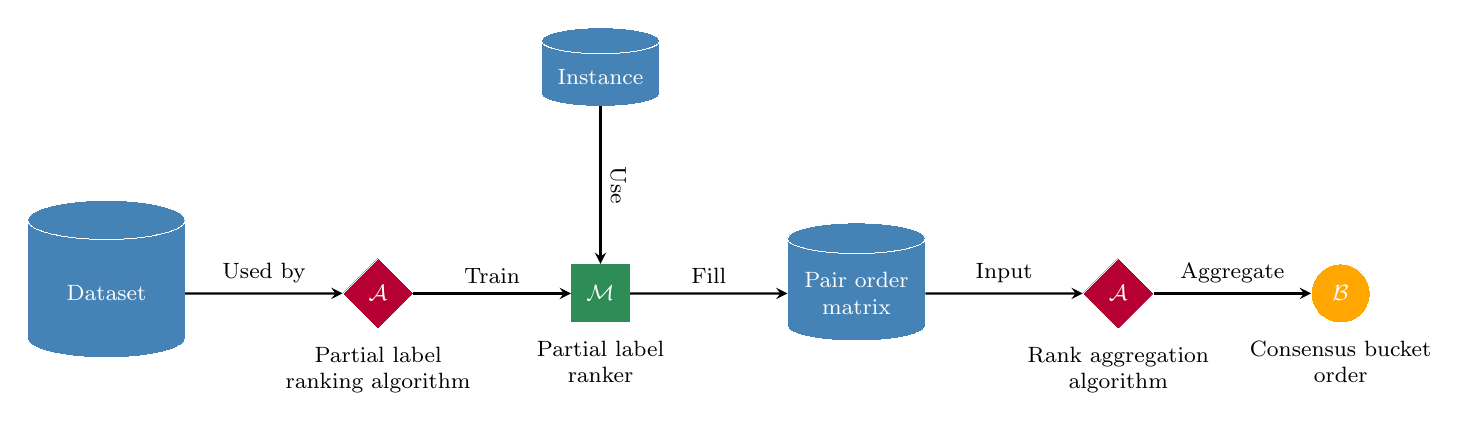
\begin{tikzpicture}[thick]

        % Modify the separation between columns
        \setlength{\tabcolsep}{0.15cm}

        % Dataset
        \node (dataset) [dataset] {Dataset};

        % Algorithm
        \node (algorithm) [algorithm, right = 2cm of dataset] {\(\mathcal{A}\)};
        \path (dataset) edge node [annotation, above] {Used by} (algorithm);
        \node [annotation, below = 0.1cm of algorithm] {Partial label\\ranking algorithm};

        % Partial label ranker
        \node (model) [function, right = 2cm of algorithm] {\(\mathcal{M}\)};
        \path (algorithm) edge node [annotation, above] {Train} (model);
        \node [annotation, below = 0.1cm of model] {Partial label\\ranker};

        % Instance
        \node (instance) [instance, above = 2cm of model] {Instance};
        \path (instance) edge node [annotation, above, sloped] {Use} (model);

        % Pair order matrix
        \node (matrix) [preference, right = 2cm of model] {Pair order\\matrix};
        \path (model) edge node [annotation, above] {Fill} (matrix);

        % Rank aggregation algorithm
        \node (aggregation) [algorithm, right = 2cm of matrix] {\(\mathcal{A}\)};
        \path (matrix) edge node [annotation, above] {Input} (aggregation);
        \node [annotation, below = 0.1cm of aggregation] {Rank aggregation\\algorithm};

        % Consensus bucket order
        \node (prediction) [prediction, right = 2cm of aggregation] {\(\B\)};
        \path (aggregation) edge node [annotation, above] {Aggregate} (prediction);
        \node [annotation, below = 0.1cm of prediction] {Consensus bucket\\order};

    \end{tikzpicture}
}

    \caption{Example of the complete learning and inference process in the partial label ranking problem}
    \label{figure:plr}
\end{figure}%
%
%

In the existing partial label ranking literature, the optimal bucket order problem is typically solved to obtain the consensus bucket order.
%
For this purpose, the current state-of-the-art method, as described in Section \ref{section:obop}, is employed.
%
Consequently, this algorithm is used as a baseline for comparing the performance of alternative aggregation~techniques.
%
%

Formally, the partial label ranking problem involves a finite set of \(n\) items to be ranked \(\I = \{1, \dots, n\}\) and a set of \(N\) training pairs \(\D = \{(x^i, \pi^i)\}_{i = 1}^{N} \subseteq \mathcal{X} \times \mathcal{S}_\I^{\succeq, \mathrm{inc}}\).
%
Here, \(\X\) denotes the instance space (typically a subset of \(\mathbb{R}^m\)) and \(\mathcal{S}_\I^{\succeq, \mathrm{inc}}\) denotes the set of (possibly incomplete) partial rankings defined over \(\mathcal{I}\).
%
Each pair \((x^i, \pi^i) \in \D\), consists of a configuration of values over \(m\) predictive features, i.e., \(x^i = (x_1^i, \dots, x_m^i)\), and a (possibly incomplete) ranking with ties of the values in \(\I\), i.e., \(\pi^{i}\). 
%
Given these, a partial label ranking algorithm learns a preference model, which is then utilized to assign a bucket order \(\B\) to any input instance \(x \in \X\).
%
%

% % % % % % % % % % Alternative rank aggregation algorithms % % % % % % % % % %
\section{Alternative rank aggregation algorithms}
\label{section:aggregations}

This section explores alternative rank aggregation methods designed to address the partial label ranking problem, providing different approaches to enhance the prediction of consensus bucket orders.

% % % % % % % % % % Scoring-based % % % % % % % % % %
\subsection{Scoring-based}
\label{section:scoring}

In \textit{scoring-based} aggregation algorithms, the primary focus is on the values within the given pair order matrix \(C\). 
%
Specifically, a scoring function \(S: \I \to \mathbb{R}\) assigns a score \(S(u)\) to each item \(u\). 
%
For most scoring functions, the score \(S(u)\) is a value that depends on the pairwise preference relations between an item \(u\) and every other item in \(\I\).
%
%

Once the scores for each item have been calculated, the items are ranked according to their respective scores, following a clear value-based ranking criterion.
%
Items are ranked in decreasing order of their scores.
%
For instance, if the score of one item \(u\) is larger than that of another item \(v\), i.e., \(S(u) > S(v)\), then \(u\) is ranked ahead of \(v\), i.e., \(u \succ v\).
%
On the other hand, if the values are the same, i.e., \(S(u) = S(v)\), then \(u\) and \(v\) are considered tied, i.e., \(u \sim v\), and are placed in the same bucket within the bucket order.
%
%
The value-based ranking criteria are precise, ensuring no ambiguous rankings and guaranteeing that a bucket order is always present in the results.
%
%

Scoring-based aggregation algorithms are often preferred for rank aggregation due to their ability to balance accuracy and computational efficiency. 
%
Next, we describe two well-known scoring-based aggregation algorithms: \textit{Copeland} and \textit{Borda}.
%
%

% % % % % % % % % % Copeland % % % % % % % % % %
\subsubsection*{Copeland}

The \textit{Copeland} aggregation algorithm (also known as \textit{Copeland ranking}) defines its scoring function \(S\) based on the total number of wins for each item in pairwise comparisons \parencite{copeland_reasonable_1951}. 
%
Specifically, an item \(u\) receives one point for winning a pairwise comparison against \(v\) if \(C(u, v) > 0.5\).
%
Nevertheless, a key drawback of this approach is that it does not account for the margin of victory.
%
To be more precise, even when \(C(u, v) - C(v, u) \approx \epsilon\) for a small \(\epsilon > 0\), \(u\) still receives a full point for winning~over~\(v\).
%
%

To address this issue, we introduce a hyperparameter \(\beta \geq 0\) to control the threshold for determining a clear winner.
%
Algorithm \ref{algorithm:copeland} provides a detailed step-by-step procedure for implementing this adaptation of the Copeland aggregation method.
%
With the introduction of \(\beta\), \(u\) earns one point for winning a pairwise comparison against \(v\) only if \(C(u, v) > 0.5 + \beta\).
%
In cases where the scores are very close, resulting a draw within the range \(0.5 - \beta \leq C(u, v) \leq 0.5 + \beta\), \(u\) earns half a point.
%
Conversely, \(u\) receives no points if \(C(u, v) < 0.5 - \beta\).
%
%

Formally, the scoring function \(S\) for an item \(u\) in our adaptation of the Copeland algorithm is computed as:
%
\begin{equation*}
S(u) = \sum_{v \in \I:v\neq u}
    \begin{cases}
        1 & \text{ if } C(u, v) > 0.5 + \beta, \\
        0.5 & \text{ if } 0.5 + \beta \geq C(u,v) \geq 0.5 - \beta, \\
        0 & \text{ if } C(u,v) < 0.5 - \beta.
    \end{cases}
\end{equation*}
%
Note that introducing the hyperparameter increases the likelihood of producing ties or buckets with the modified Copeland aggregation method.
%
This, in turn, enhances its suitability for the more general partial label ranking problem.
%
%

% % % % % % % % % % Borda % % % % % % % % % %
\subsubsection*{Borda}

The fundamental concept of the \textit{Borda} aggregation algorithm (also known as \textit{Borda ranking}) is, roughly speaking, by ranking items by their average probability of being preferred over another uniformly at randomly chosen item \parencite{black_partial_1976}.
%
Formally, the scoring function \(S\) in Borda is thus defined as:
%
\begin{equation*}
    B(u) = \frac{1}{n-1}\sum_{v \in \I:v\neq u} C(u, v).
\end{equation*}
%
For the sake of convenience, we will omit the normalizing factor \(\nicefrac{1}{n-1}\), as this does not change the ordering.
%
%

The main problem with this approach lies in the sorting procedure: items are assigned the same rank if and only if they have the exact same score.
%
This strict criterion makes it unlikely for items to be grouped in the same bucket, even when their scores are close, often resulting in bucket orders that are nearly total orders.
%
To mitigate this issue, we once again introduce a hyperparameter \(\beta \geq 0\) for this issue in order to relax the grouping criterion. 
%
The idea is to place items in the same bucket if the difference between their scores falls within the range defined by \(\beta\).
%
Specifically, for two items \(u\) and \(v\), if \(S(u) - S(v) \in [-\beta, \beta]\), then \(u \sim v\).
%
This mechanism naturally extends to multiple items through a \textit{cascading effect}, ensuring that items with closely related scores are consistently placed into the same bucket.
%
Algorithm \ref{algorithm:borda} illustrates the detailed step-by-step implementation of this~approach.
%
%

It is worth pointing out that the computational complexity for scoring from the pair order matrix is \(\mathcal{O}(n^{2})\) for both scoring-based algorithms.
%
On the other hand, they exhibit \(O(n\log n)\) complexity in the sorting phase.
%
Finally, it is worth mentioning that both classical variants of the Copeland or the Borda aggregation methods can be recovered by setting the introduced hyperparameter \(\beta\) to zero.
%

% % % % % % % % % % Probabilistic-based % % % % % % % % % %
\subsection{Probabilistic-based}
\label{section:probabilistic}

% % % % % % % % % % Markov chain % % % % % % % % % %
\subsubsection*{Markov chain}

Four variations of the \textit{Markov chain} algorithms have been developed to address the rank aggregation problem \parencite{dwork_rank_2001}.
%
The primary objective of these algorithms is to generate an aggregated ranking that minimizes the influence of items that are spuriously ranked highly in only a minority of lists. 
%
%

The algorithms begin by representing a Markov chain with undirected edges.
%
Each Markov chain is defined by an \(n \times n\) \textit{transition matrix} \(P\), where \(P(u, v)\) represents the transition probabilities from state \(u\) to state \(v\).
%
The transitioning mechanism varies across the different algorithms; that is, the pattern of state transitions in the constructed Markov chain is not uniform.
%
In particular, upon reaching state \(u\), the next state \(v\) is selected as follows:
%
\begin{itemize}
    %
    \item in \textit{Markov chain 1}, uniformly at random from the set of items ranked at least as high as \(u\) in at least one input ranking;
    %
    \item in \textit{Markov chain 2}, by first picking a random input ranking and then choosing \(v\) uniformly at random from the set of items ranked at least as high as \(i\) in that ranking;
    %
    \item in \textit{Markov chain 3}, by choosing a random item \(v\) from a random input ranking;
    %
    \item in \textit{Markov chain 4}, uniformly at random
    %
\end{itemize}
%
%

One limitation of the first three Markov chain algorithms is that their transition matrix computations rely on a set of rankings and cannot be derived directly from the pair order matrix (see Algorithms \ref{algorithm:mc1}, \ref{algorithm:mc2}, and \ref{algorithm:mc3} for the details).
%
In contrast, Markov chain 4 (Algorithm \ref{algorithm:mc4}) allows the direct computation of each entry \(P(u, v)\) in the transition matrix from a given pair order matrix \(C\), using the following formulation:
%
\begin{equation*}
    P(u, v) =
        \begin{cases}
                \frac{1}{n} & \text{ if } u \neq v \land C(u, v) \leq 0.5, \\
                0 & \text{ if } u \neq v \land C(u, v) > 0.5, \\
                1 - \sum_{w:w \neq u} P(u, v) & \text{ if } u = w.
        \end{cases}
\end{equation*}
%
This direct computation provides an advantage for Markov chain 4 when only a pair order matrix is available \parencite{alfaro_pairwise_2023, alfaro_multi-dimensional_2023}.
%
To evaluate these algorithms, we employed a partial label ranker capable of predicting both, the pair order matrix and the subset of (possibly incomplete) partial rankings required to derive it.
%
%

Once the Markov chain with the transition matrix is constructed, the algorithms will run on this chain until convergence.
%
Subsequently, the last step is to find the stationary distribution \(x\) of this Markov chain that satisfies 
%
\begin{equation*}
    x = xP. 
\end{equation*}
%
%

After getting the stationary distribution
%
\begin{equation*}
    x =
    \begin{pmatrix}
        x_{1} \\
        \dots \\
        x_{n}
    \end{pmatrix},
\end{equation*}
%
the items are ranked in decreasing order of their value in \(x\), with equal values resulting in tied items.
%
%
As stated by \textcite{dwork_rank_2001}, all Markov chain methods take about \(\Theta(n^2N + n^3)\) time.
%
However, in practice, it can be reduced to \(\mathcal{O}(n^2N)\) if the transition matrix is explicitly computed.
%
%

% % % % % % % % % % Maximal lottery % % % % % % % % % %
\subsubsection*{Maximal lottery}

The \textit{maximal lottery} algorithm is inspired by the concept introduced by \textcite{fishburn_probabilistic_1984}. 
%
In this \textit{game-theoretic} model, the set of items \(\I\) is treated as a set of alternatives.
%
Let
%
\begin{equation*}
    \Delta(\I) = \left\{p \in \left[0, 1\right]^{\I} : \sum_{x \in \I}  p(x) = 1\right\}
\end{equation*}
%
be the set of all lotteries over alternatives, where \(p(x)\) corresponds to the probability of selecting the alternative \(x\).
%
The pair order matrix \(C\) is converted into a comparison matrix \(M\) by assigning \(M(u, v) = C(u, v)\), for all \(u, v \in \I\) where \(u \neq v\); and setting \(M(u, u) = 0\), for all \(u \in \I\).
%
The comparison matrix \(M\) then induces a skew-symmetric matrix defined as
%
\begin{equation*}
    \widetilde{M} = M - M^{T}.
\end{equation*}
%
In game theory, \(\widetilde{M}\) can be interpreted as a symmetric zero-sum game.
%
%

According to the \textit{minimax} theorem \parencite{von_mathematische_1928}, there exists a lottery
%
\begin{equation*}
p_{max} = 
    \begin{pmatrix}
        p_{1} \\
        \dots \\
        p_{n}
    \end{pmatrix},
\end{equation*}
%
that performs at least as well as any other lottery, meaning:
%
\begin{equation*}
    \exists p_{max} \in \Delta(\I) : p_{max}^{T}\widetilde{M} \ge 0.
\end{equation*}
%
This lottery, \(p_{max}\), is referred to as the maximal lottery.
%
After computing \(p_{max}\), the items are ranked in decreasing order of their values in \(p_{max}\), with ties occurring if the values are equal.
%
Algorithm \ref{algorithm:ml} presents the pseudocode for developing this algorithm.
%
%

The problem of finding the maximal lottery can be expressed as \textit{linear programming} task \parencite{von_mathematische_1928}. 
%
To address this efficiently, researchers have developed various strategies to solve the problem effectively \parencite{daskalakis_complexity_2009}. %
%
%

% % % % % % % % % % Experimental evaluation % % % % % % % % % %
\section{Experimental evaluation}
\label{section:experiments}

This section presents an empirical evaluation of the alternative rank aggregation algorithms, focusing on assessing their performance in addressing the partial label ranking problem.

% % % % % % % % % % Methodology % % % % % % % % % %
\subsection{Methodology}

The metric of interest is the \(\tau_X\) \textit{rank correlation coefficient} \parencite{emond_new_2002}.
%
Similar to how \textit{Kendall's} \(\tau\) is used for label ranking \parencite{cheng_2009_decision}, \(\tau_X\) is specifically designed to deal with tied rankings.
%
As a result, it is a valuable and widely adopted metric for evaluating partial label ranking performance \parencite{alfaro_learning_2021}.
%
The algorithms were evaluated using five repetitions of a ten-fold (\(5 \times 10\)) cross-validation method.
%
To assess their robustness against incomplete information, 0\%, 30\%, and 60\% of class label positions were randomly omitted.
% 
These percentages are standard values used for label and partial label ranking problems \parencite{cheng_label_2010, alfaro_learning_2021, alfaro_ensemble_2023}.
%
Finally, the results were analyzed following the procedure outlined in \parencite{demsar_statistical_2006, garcia_extension_2008} using the \texttt{exreport} software tool \parencite{arias_exreport:_2015}.
%
Initially, a \textit{Friedman test} \parencite{friedman_comparison_1940} was conducted to evaluate the null hypothesis that all algorithms exhibit equal performance.
%
Upon rejection of this hypothesis, a post-hoc analysis employing \textit{Holm's procedure} \parencite{holm_simple_1979} was carried out to compare each algorithm against the top-ranked one identified by the Friedman test.
%
The Friedman test and the post-hoc analysis were performed at a 5\% significance level.

% % % % % % % % % % Datasets % % % % % % % % % %
\subsection{Datasets}

Table \ref{table:datasets} provides an overview of the datasets included in the experimental evaluation and their respective properties.
%
The datasets above the dashed line are synthetic and derived by transforming multi-class datasets from the UCI repository \parencite{kelly_uci} into partial label ranking data using the procedure outlined in \parencite{alfaro_learning_2021}.
%
In contrast, the datasets below the dashed line represent real-world scenarios \parencite{kelly_uci, maxwell_movielens_2016} and originate from natural partial label ranking problems.
%
%

The columns display the following information: Identifier; which corresponds to the unique identifier of the dataset in the \texttt{OpenML} repository \parencite{vanschoren_openml_2014}, \#of instances; representing the total number of instances in the dataset; \#of features, indicating the number of input variables describing each instance; \#of classes, specifying the total number of class labels included in the ranking problem; Unique \#of rankings, which denotes the number of distinct partial label rankings present in the dataset; and Mean \#of buckets, representing the average number of buckets within each ranking.

\begin{table*}
    \centering
    \caption{Description of the datasets}
    \label{table:datasets}
    \resizebox{\textwidth}{!}
    {%
        \begin{tabular}{lrrrrrr}
            \toprule
            Dataset & Identifier & \#of instances & \#of features & \#of classes & Unique \#of rankings & Mean \#of buckets \\
            \midrule
            authorship & 42835 & 841 & 70 & 4 & 47 & 3.063 \\
            blocks & 42836 & 5472 & 10 & 5 & 116 & 2.337 \\
            breast & 42838 & 109 & 9 & 6 & 62 & 3.925 \\
            ecoli & 42844 & 336 & 7 & 8 & 179 & 4.140 \\
            glass & 42848 & 214 & 9 & 6 & 105 & 4.089 \\
            iris  & 42871 & 150 & 4 & 3 & 7 & 2.380 \\
            letter & 42853 & 20000 & 16 & 26 & 15014 & 7.033 \\
            libras & 42855 & 360 & 90 & 15 & 356 & 6.889 \\
            pendigits & 42857 & 10992 & 16 & 10 & 3327 & 3.397 \\
            satimage & 42858 & 6435 & 36 & 6 & 504 & 3.356 \\
            segment & 42860 & 2310 & 18 & 7 & 271 & 3.031 \\
            vehicle & 42864 & 846 & 18 & 4 & 47 & 3.117 \\
            vowel & 42866 & 528 & 10 & 11 & 504 & 5.739 \\
            wine & 42872 & 178 & 13 & 3 & 11 & 2.680 \\
            yeast & 42870 & 1484 & 8 & 10 & 1006 & 5.929\\[0.1cm]
            \hdashline
            \\[-0.35cm]
            algae & 45755 & 316 & 18 & 7 & 316 & 4.877 \\
            movies & 45738 & 260 & 64 & 15 & 260 & 3.046 \\
            \bottomrule
        \end{tabular}
    }
\end{table*}

% % % % % % % % % % Learning methods % % % % % % % % % %
\subsection{Learning methods}
\label{section:algorithms}

We utilized the \textit{partial label ranking trees} algorithm with the \textit{entropy} criterion \parencite{alfaro_learning_2021} as the base learning method.
%
This configuration ensures that all aggregation techniques share the same decision tree structure, learned independently of the consensus bucket order.
%
The differences lie solely in the bucket orders assigned to the leaf nodes during the learning phase, which are determined by the respective aggregation technique.
%
In other words, the focus here is explicitly on the aggregation step (see Fig. \ref{figure:plr}), enabling a targeted investigation into the influence of the chosen aggregation method.
%
%

As explained in Section \ref{section:scoring}, the Borda and Copeland algorithms incorporate a \(\beta\) hyperparameter to manage the items ranked in the same position.
%
This occurs when their respective scores fall within the overlap range defined by \(\beta\).
%
As expected, this hyperparameter has a significant impact on the performance of the methods.
%
To investigate this, we conducted a preliminary experiment to analyze its effect.
%
In particular, we tested \(\beta\) values ranging from 0 to 2 on the synthetic datasets to identify the value that achieves the best average performance across these datasets.
%
Note that real-world datasets were not used in this analysis, as a different procedure, outlined in Section \ref{section:real}, will be employed to determine the \(\beta\) value for those datasets.
%
%

Fig. \ref{figure:beta} illustrates the impact of the \(\beta\) hyperparameter on the \(\tau_X\) score for the Borda and Copeland algorithms.
%
Notably, the optimal \(\beta\) value is 0.9 for Borda and 0.4 for Copeland, irrespective of the percentage of missing class label positions.
%
Indeed, as the \(\beta\) value increases, the techniques become more prone to grouping items into the same bucket, with the extreme case being all items placed in a single bucket.
%
For Copeland, this critical point occurs at \(\beta = 0.5\) because the scoring function assigns all items a score of 0.5.
%
This occurs because all values in the pair order matrix fall within the range \([0.5 - \beta, 0.5 + \beta] = [0, 1]\), which coincides with the full range of the pair order matrix, as described in Section \ref{section:obop}.

 \begin{figure}
    \centering
    \includegraphics[width = 0.7\textwidth]{figures/Fig2.pdf}
    \caption{Average \(\tau_X\) score across datasets for varying \(\beta\) values, comparing the algorithms at different percentages of missing class label positions}
    \label{figure:beta}
\end{figure}

% % % % % % % % % % Results % % % % % % % % % %
\subsection{Results}

This section presents the results of our experimental evaluation on both synthetic and real-world datasets.
%
The aggregation methods described in Section \ref{section:aggregations} are denoted by their respective name.
%
In constrast, the representative aggregation method for the optimal bucket order problem is the bucket pivot algorithm (see Section \ref{section:obop}) and consequently denoted by \textit{Bucket pivot} in the upcoming figures.

% % % % % % % % % % Synthetic datasets % % % % % % % % % %
\subsubsection{Synthetic datasets}
\label{section:synthetic}

Table \ref{table:holm} summarizes the statistical test outcomes, where boldfaced values denote the algorithms that are not statistically significantly different from the one ranked first according to the Friedman test.
%
The columns are as follows: Rank, indicating the average rank position assigned by the Friedman test; P-value, showing the \(p\)-value adjusted using the Holm's procedure; and Win, Tie, and Loss, representing the number of times that the control algorithm wins, ties and loses to the respective algorithm.
%
Additionally, Appendix \ref{section:complete} contains the complete results of the cross-validation study for scenarios with 0\%, 30\%, and 60\% of missing class label positions.
%
In these tables, the underlined values indicate the algorithm(s) that achieved the highest \(\tau_X\) score.
%
Boldfaced values, meanwhile, denote algorithms whose confidence intervals, defined by their mean and standard deviation, overlap with the interval of the best-performing~algorithm.
%
%

This analysis reveals that the scoring-based methods perform remarkably well in all the scenarios.
%
Moreover, with incomplete rankings, the Borda algorithm outperforms the bucket pivot method when 30\% of missing class label positions are missing.
%
As the percentage of missing class label positions increases, both Borda and Copeland demonstrate greater robustness compared to other methods, consistently ranking ahead of the bucket pivot method.
%
This trend is particularly evident with 60\% of missing data, where Borda and Copeland exhibit significantly better performance, as shown in Fig. \ref{figure:accuracy}.
%
In contrast, the probabilistic-based methods exhibit significantly weaker performance across all scenarios, consistently ranking lower than the scoring-based algorithms.
%
%

\begin{table*}
    \setlength{\tabcolsep}{0.15cm}
    \centering
    \caption{Friedman's and Holm's tests with varying miss probability}
    \label{table:holm}
    \resizebox{\textwidth}{!}
    {%
        % 0%
        \begin{tabu}{|[0.05cm]lrrrrr|}
            \tabucline[0.05cm]{-}
            \multicolumn{6}{|[0.05cm]c|}{\textbf{Missing percentage: 0\%}} \\
            \hline
            \multicolumn{6}{|[0.05cm]c|}{Friedman p-value: \(\bf 5.431 \times 10^{-18}\)} \\
            \hline
            \multicolumn{6}{|[0.05cm]c|}{Holm results} \\
            \hline
            Method & Rank & P-value & Win & Tie & Loss \\
            \hline
            Bucket pivot & 1.53 & - & - & - & \\
            Borda & 2.03 & \(\bf 5.52 \times 10^{-1}\) & 10 & 1 & 6 \\
            Copeland & 2.68 & \(\bf 3.44 \times 10^{-1}\) & 14 & 1 & 2 \\
            Markov chain 3 & 4.82 & \(2.65 \times 10^{-4}\) & 17 & 0 & 0 \\
            Markov chain 1 & 5.26 & \(3.50 \times 10^{-5}\) & 17 & 0 & 0 \\
            Markov chain 2 & 5.44 & \(1.61 \times 10^{-5}\) & 17 & 0 & 0 \\
            Markov chain 4 & 6.59 & \(1.04 \times 10^{-8}\) & 17 & 0 & 0 \\
            Maximal lottery & 7.65 & \(2.31 \times 10^{-12}\) & 17 & 0 & 0 \\
            \tabucline[0.05cm]{-}
        \end{tabu}%
        % 30%
        \begin{tabu}{lrrrrr}
            \tabucline[0.05cm]{-}
            \multicolumn{6}{c|}{\textbf{Missing percentage: 30\%}} \\
            \hline
            \multicolumn{6}{c|}{Friedman p-value: \(\bf 2.033 \times 10^{-18}\)} \\
            \hline
            \multicolumn{6}{c|}{Holm results} \\
            \hline
            Method & Rank & P-value & Win & Tie & Loss \\
            \hline
            Borda & 1.44 & - & - & - & \\
            Bucket pivot & 2.09 & \(\bf 4.41 \times 10^{-1}\) & 12 & 1 & 4 \\
            Copeland & 2.82 & \(\bf 2.00 \times 10^{-1}\) & 15 & 0 & 2 \\
            Markov chain 3 & 4.38 & \(1.40 \times 10^{-3}\) & 17 & 0 & 0 \\
            Markov chain 2 & 5.09 & \(5.68 \times 10^{-5}\) & 17 & 0 & 0 \\
            Markov chain 1 & 5.71 & \(1.93 \times 10^{-6}\) & 17 & 0 & 0 \\
            Markov chain 4 & 7.06 & \(1.37 \times 10^{-10}\) & 17 & 0 & 0 \\
            Maximal lottery & 7.41 & \(8.34 \times 10^{-10}\) & 16 & 0 & 1 \\
            \tabucline[0.05cm]{-}
        \end{tabu}%
        % 60%
        \begin{tabu}{|lrrrrr|[0.05cm]}
            \tabucline[0.05cm]{-}
            \multicolumn{6}{c|[0.05cm]}{\textbf{Missing percentage: 60\%}} \\
            \hline
            \multicolumn{6}{c|[0.05cm]}{Friedman p-value: \(\bf 1.043 \times 10^{-13}\)} \\
            \hline
            \multicolumn{6}{c|[0.05cm]}{Holm results} \\
            \hline
            Method & Rank & P-value & Win & Tie & Loss \\
            \hline
            Borda & 1.35 & - & - & - & \\
            Copeland & 2.88 & \(\bf 1.37 \times 10^{-1}\) & 15 & 0 & 2 \\
            Bucket pivot & 2.88 & \(\bf 1.35 \times 10^{-1}\) & 14 & 0 & 3 \\
            Markov chain 3 & 4.26 & \(1.59 \times 10^{-3}\) & 17 & 0 & 0 \\
            Markov chain 2 & 5.76 & \(6.25 \times 10^{-7}\) & 17 & 0 & 0 \\
            Markov chain 1 & 5.79 & \(6.25 \times 10^{-7}\) & 17 & 0 & 0 \\
            Maximal lottery & 6.47 & \(6.72 \times 10^{-9}\) & 16 & 0 & 1 \\
            Markov chain 4 & 6.59 & \(3.24 \times 10^{-9}\) & 17 & 0 & 0 \\
            \tabucline[0.05cm]{-}
        \end{tabu}%
    }
\end{table*}
%
%

\begin{figure}
    \centering
    \includegraphics[width = 0.7\textwidth]{figures/Fig3.pdf}
    \caption{Average \(\tau_X\) score across datasets for varying percentages of missing class label positions, comparing the algorithms}
    \label{figure:accuracy}
\end{figure}
%
%

The accuracy metric (i.e., the \(\tau_X\) rank correlation coefficient) penalizes in two specific scenarios: %
%
\begin{enumerate*}[label = (\roman*)]%
%
    \item when items that are ranked ahead or tied in the true ranking are placed behind in the predicted ranking, and %
    %
    \item when items ranked behind in the true ranking are tied in the predicted ranking. %
    %
\end{enumerate*} %
%
Based on this, we hypothesized that the algorithms either produce too few buckets, which prevents them from correctly identifying tied items or generate too many buckets, making it difficult to determine whether one item is ranked behind another accurately.
%
Both scenarios lead to penalties in the scoring metric.
%
To investigate this, we measured the discrepancy between the number of buckets in the predicted and true bucket orders, as illustrated in Fig. \ref{figure:buckets}, where the x-axis is arranged based on the datasets' mean number of buckets. 
%
Notably, the probabilistic-based methods exhibit more pronounced deviations compared to scoring-based algorithms.
%
Specifically, Markov chain 1, 2, and 3 methods tend to produce bucket orders with excessive buckets in datasets with a higher number of class labels (e.g., yeast, libras, and letter), essentially approximating total orders.
%
On the other hand, Markov chain 4 and the maximal lottery algorithm often generate bucket orders with too few buckets, typically resulting in one clearly defined top bucket while grouping the remaining items into a small number of broader, less refined buckets.
%
In other scenarios, all probabilistic-based methods tend to produce bucket orders with fewer buckets overall.
%
%

\begin{figure}
    \centering
    \includegraphics[width = \textwidth]{figures/Fig4.pdf}
    \caption{Difference in the number of buckets between the true and predicted bucket orders for each algorithm and dataset with varying percentages of missing class label positions}
    \label{figure:buckets}
\end{figure}
%
%

Regarding computational complexity, the training times (in seconds) are presented in Table \ref{table:time}.
%
Only the scoring-based algorithms and the bucket pivot method are included due to the low accuracy of the probabilistic-based methods and their significantly higher computational demands.
%
Additionally, prediction times are not included because they are identical across all algorithms.
%
This is because the underlying decision tree structure is the same for all the methods, as explained in Section \ref{section:algorithms}.
%
In general, the Borda and Copeland methods are approximately twice as fast as the bucket pivot algorithm, despite the latter having a lower computational complexity, as stated in Sections \ref{section:obop} and \ref{section:scoring}.
%
This discrepancy can likely be attributed to the recursive nature of the bucket pivot method, which introduces additional overhead, thereby increasing its practical runtime.

\begin{table*}
    \centering
    \caption{Average training times (mean and standard deviation, in seconds) for the scoring-based algorithms (Borda and Copeland) and the bucket pivot method across datasets with missing class label positions}
    \label{table:time}
    \resizebox{\textwidth}{!}
     & \multicolumn{3}{c}{30\%} & \multicolumn{3}{c}{60\%} \\
            \cmidrule{2-10}
            & Bucket pivot & Borda & Copeland & Bucket pivot & Borda & Copeland & Bucket pivot & Borda & Copeland \\
            \midrule
            authorship & 0.678 $ \pm $ 0.024 & 0.341 $ \pm $ 0.013 & 0.341 $ \pm $ 0.013 & 0.537 $ \pm $ 0.021 & 0.294 $ \pm $ 0.019 & 0.282 $ \pm $ 0.009 & 0.317 $ \pm $ 0.022 & 0.186 $ \pm $ 0.013 & 0.186 $ \pm $ 0.010 \\
            blocks & 1.232 $ \pm $ 0.050 & 0.697 $ \pm $ 0.034 & 0.695 $ \pm $ 0.031 & 1.142 $ \pm $ 0.065 & 0.638 $ \pm $ 0.038 & 0.646 $ \pm $ 0.043 & 0.852 $ \pm $ 0.061 & 0.480 $ \pm $ 0.034 & 0.481 $ \pm $ 0.036 \\
            breast & 0.027 $ \pm $ 0.003 & 0.014 $ \pm $ 0.002 & 0.014 $ \pm $ 0.002 & 0.023 $ \pm $ 0.002 & 0.012 $ \pm $ 0.002 & 0.013 $ \pm $ 0.001 & 0.018 $ \pm $ 0.002 & 0.009 $ \pm $ 0.001 & 0.010 $ \pm $ 0.001 \\
            ecoli & 0.045 $ \pm $ 0.004 & 0.027 $ \pm $ 0.002 & 0.028 $ \pm $ 0.003 & 0.041 $ \pm $ 0.003 & 0.025 $ \pm $ 0.002 & 0.025 $ \pm $ 0.002 & 0.032 $ \pm $ 0.003 & 0.020 $ \pm $ 0.003 & 0.020 $ \pm $ 0.002 \\
            glass & 0.051 $ \pm $ 0.004 & 0.024 $ \pm $ 0.003 & 0.024 $ \pm $ 0.002 & 0.047 $ \pm $ 0.004 & 0.022 $ \pm $ 0.003 & 0.023 $ \pm $ 0.002 & 0.034 $ \pm $ 0.004 & 0.017 $ \pm $ 0.002 & 0.017 $ \pm $ 0.002 \\
            iris & 0.007 $ \pm $ 0.002 & 0.005 $ \pm $ 0.002 & 0.005 $ \pm $ 0.002 & 0.005 $ \pm $ 0.001 & 0.004 $ \pm $ 0.001 & 0.004 $ \pm $ 0.001 & 0.004 $ \pm $ 0.001 & 0.004 $ \pm $ 0.002 & 0.003 $ \pm $ 0.001 \\
            letter & 18.073 $ \pm $ 0.119 & 17.501 $ \pm $ 0.134 & 17.554 $ \pm $ 0.137 & 14.820 $ \pm $ 0.104 & 14.454 $ \pm $ 0.100 & 14.517 $ \pm $ 0.112 & 9.771 $ \pm $ 0.107 & 9.409 $ \pm $ 0.112 & 9.539 $ \pm $ 0.088 \\
            libras & 2.121 $ \pm $ 0.063 & 1.640 $ \pm $ 0.047 & 1.685 $ \pm $ 0.044 & 2.004 $ \pm $ 0.080 & 1.536 $ \pm $ 0.059 & 1.589 $ \pm $ 0.059 & 1.521 $ \pm $ 0.047 & 1.135 $ \pm $ 0.044 & 1.183 $ \pm $ 0.036 \\
            pendigits & 4.848 $ \pm $ 0.060 & 3.433 $ \pm $ 0.044 & 3.434 $ \pm $ 0.049 & 4.810 $ \pm $ 0.061 & 3.498 $ \pm $ 0.049 & 3.512 $ \pm $ 0.052 & 3.553 $ \pm $ 0.036 & 2.578 $ \pm $ 0.043 & 2.662 $ \pm $ 0.082 \\
            satimage & 3.527 $ \pm $ 0.063 & 2.050 $ \pm $ 0.039 & 2.053 $ \pm $ 0.039 & 3.151 $ \pm $ 0.058 & 1.895 $ \pm $ 0.039 & 1.887 $ \pm $ 0.030 & 2.235 $ \pm $ 0.035 & 1.409 $ \pm $ 0.028 & 1.424 $ \pm $ 0.033 \\
            segment & 1.300 $ \pm $ 0.033 & 0.682 $ \pm $ 0.017 & 0.689 $ \pm $ 0.021 & 1.199 $ \pm $ 0.038 & 0.635 $ \pm $ 0.017 & 0.640 $ \pm $ 0.020 & 0.932 $ \pm $ 0.036 & 0.493 $ \pm $ 0.015 & 0.499 $ \pm $ 0.017 \\
            vehicle & 0.228 $ \pm $ 0.013 & 0.118 $ \pm $ 0.009 & 0.122 $ \pm $ 0.009 & 0.192 $ \pm $ 0.010 & 0.101 $ \pm $ 0.007 & 0.104 $ \pm $ 0.008 & 0.122 $ \pm $ 0.006 & 0.068 $ \pm $ 0.004 & 0.069 $ \pm $ 0.004 \\
            vowel & 0.338 $ \pm $ 0.012 & 0.230 $ \pm $ 0.009 & 0.234 $ \pm $ 0.011 & 0.331 $ \pm $ 0.013 & 0.215 $ \pm $ 0.009 & 0.224 $ \pm $ 0.008 & 0.268 $ \pm $ 0.009 & 0.171 $ \pm $ 0.007 & 0.178 $ \pm $ 0.007 \\
            wine & 0.041 $ \pm $ 0.004 & 0.018 $ \pm $ 0.002 & 0.020 $ \pm $ 0.006 & 0.030 $ \pm $ 0.003 & 0.015 $ \pm $ 0.003 & 0.014 $ \pm $ 0.002 & 0.018 $ \pm $ 0.002 & 0.009 $ \pm $ 0.002 & 0.009 $ \pm $ 0.002 \\
            yeast & 0.256 $ \pm $ 0.011 & 0.161 $ \pm $ 0.010 & 0.162 $ \pm $ 0.008 & 0.256 $ \pm $ 0.016 & 0.166 $ \pm $ 0.012 & 0.167 $ \pm $ 0.009 & 0.191 $ \pm $ 0.009 & 0.123 $ \pm $ 0.006 & 0.125 $ \pm $ 0.004 \\
            \bottomrule
        \end{tabular}
    }
\end{table*}

% % % % % % % % % % Real-world datasets % % % % % % % % % %
\subsubsection{Real-world datasets}
\label{section:real}

The preliminary analysis regarding the \(\beta\) hyperparameter in Section \ref{section:algorithms} has shown that the selected value is crucial for the performance of the scoring-based algorithms.
%
While the analysis suggests that a fixed value might be suitable across all datasets, it is compelling to establish a criterion for selecting appropriate values when addressing real-world datasets.
%
This section introduces a recommendation system based on the experimental results with the synthetic datasets.
%
%

We trained a linear regression model using the following meta-features of the datasets as predictors for the new datasets: the number of instances, the number of features, the number of classes, the average number of buckets, and the average proportion of missing class labels.
%
Thus, each row in the training dataset represents a unique combination of a dataset and a specific percentage of missing class label positions, with percentages ranging from 0 to 60 in increments of 10.
%
These averages were computed from the \(5 \times 10\) cross-validation method carried out.
%
The target variable for the model was \(\beta\), which represents the \(\beta\) value that achieved the best average results.
%
%

Table \ref{table:real} shows the results obtained from the cross-validation study, where \(^*\) indicates that the results correspond to the best identified for the respective algorithm during the cross-validation.
%
In contrast, Table \ref{table:beta} compares the best \(\beta\) values with those predicted by the linear regression model.
%
For the algae dataset, the Borda algorithm outperforms the bucket pivot method and achieves results similar to Borda\(^*\), as the predicted \(\beta\) value is very close to the best one.
%
In the case of the Copeland algorithm, although it does not surpass the bucket pivot method, the predicted \(\beta\) value remains close to the best one.
%
On the other hand, the probabilistic-based algorithms fail to produce competitive results.
%
For the movies dataset, neither Borda nor Copeland delivers competitive results, as their predicted \(\beta\) values are not close to their respective best values.
%
Interestingly, the maximal lottery algorithm performs better than Borda and Copeland, yet it still fails to achieve the performance achieved by bucket pivot.

\begin{table*}
    \centering
    \caption{\(\tau_X\) score (mean and standard deviation) of algorithms for the real-world datasets}
    \label{table:real}
    \resizebox{\textwidth}{!}
    {
        \begin{tabular}{lrrrrrr}
            \toprule
            \multirow{2}{*}{Algorithm} & \multicolumn{3}{c}{algae} & \multicolumn{3}{c}{movies} \\
            \cmidrule{2-7}
            & 0\% & 30\% & 60\% & 0\% & 30\% & 60\% \\
            \midrule
            Bucket pivot & 0.419 $ \pm $ 0.064 & 0.381 $ \pm $ 0.049 & 0.285 $ \pm $ 0.052 & 0.439 $ \pm $ 0.032 & 0.433 $ \pm $ 0.032 & 0.433 $ \pm $ 0.029 \\
            Borda & 0.435 $ \pm $ 0.064 & 0.389 $ \pm $ 0.057 & 0.326 $ \pm $ 0.055 & 0.401 $ \pm $ 0.033 & 0.380 $ \pm $ 0.030 & 0.373 $ \pm $ 0.039 \\
            Borda\(^*\) & 0.437 $ \pm $ 0.064 & 0.395 $ \pm $ 0.059 & 0.330 $ \pm $ 0.054 & 0.437 $ \pm $ 0.027 & 0.440 $ \pm $ 0.028 & 0.442 $ \pm $ 0.025 \\
            Copeland & 0.414 $ \pm $ 0.065 & 0.362 $ \pm $ 0.055 & 0.283 $ \pm $ 0.052 & 0.265 $ \pm $ 0.038 & 0.192 $ \pm $ 0.032 & 0.180 $ \pm $ 0.037 \\
            Copeland\(^*\) & 0.420 $ \pm $ 0.065 & 0.361 $ \pm $ 0.056 & 0.286 $ \pm $ 0.053 & 0.443 $ \pm $ 0.028 & 0.443 $ \pm $ 0.028 & 0.443 $ \pm $ 0.028 \\
            Markov chain 1 & 0.390 $ \pm $ 0.060 & 0.344 $ \pm $ 0.058 & 0.294 $ \pm $ 0.065 & 0.179 $ \pm $ 0.036 & 0.135 $ \pm $ 0.032 & 0.126 $ \pm $ 0.036 \\
            Markov chain 2 & 0.384 $ \pm $ 0.059 & 0.348 $ \pm $ 0.056 & 0.293 $ \pm $ 0.069 & 0.180 $ \pm $ 0.036 & 0.145 $ \pm $ 0.032 & 0.136 $ \pm $ 0.038 \\
            Markov chain 3 & 0.394 $ \pm $ 0.058 & 0.355 $ \pm $ 0.057 & 0.300 $ \pm $ 0.067 & 0.179 $ \pm $ 0.036 & 0.147 $ \pm $ 0.032 & 0.138 $ \pm $ 0.038 \\
            Markov chain 4 & 0.364 $ \pm $ 0.057 & 0.339 $ \pm $ 0.064 & 0.275 $ \pm $ 0.053 & 0.385 $ \pm $ 0.028 & 0.250 $ \pm $ 0.041 & 0.165 $ \pm $ 0.039 \\
            Maximal lottery & 0.348 $ \pm $ 0.055 & 0.328 $ \pm $ 0.055 & 0.299 $ \pm $ 0.057 & 0.411 $ \pm $ 0.025 & 0.398 $ \pm $ 0.025 & 0.377 $ \pm $ 0.033 \\
            \bottomrule
        \end{tabular}
    }
\end{table*}

\begin{table*}
    \centering
    \caption{Comparison of the best and predicted \(\beta\) values for the scoring-based algorithms across different datasets and levels of missing class label positions}
    \label{table:beta}
    \resizebox{\textwidth}{!}
    {%
        \begin{tabular}{llrrrrrr}
            \toprule
            \multicolumn{2}{c}{\multirow{2}{*}{Algorithm}} & \multicolumn{3}{c}{algae} & \multicolumn{3}{c}{movies} \\
            \cmidrule{3-8}
            & & 0\% & 30\% & 60\% & 0\% & 30\% & 60\% \\
            \midrule
            \multirow{2}{*}{Borda} & Best & 0.8 & 0.8 & 0.8 & 1.9 & 2.0 & 2.0 \\
            & Predicted & 0.677 $ \pm $ 0.002 & 0.652 $ \pm $ 0.002 & 0.634 $ \pm $ 0.002 & 1.145 $ \pm $ 0.001 & 1.063 $ \pm $ 0.003 & 0.993 $ \pm $ 0.003 \\
            \midrule
            \multirow{2}{*}{Copeland} & Best & 0.2 & 0.3 & 0.3 & 0.5 & 0.5 & 0.5 \\
            & Predicted & 0.303 $ \pm $ 0.00 & 0.266 $ \pm $ 0.001 & 0.229 $ \pm $ 0.001 & 0.273 $ \pm $ 0.000 & 0.226 $ \pm $ 0.001 & 0.181 $ \pm $ 0.001 \\
            \bottomrule
        \end{tabular}
    }
\end{table*}

% % % % % % % % % % Conclusion % % % % % % % % % %
\section{Conclusions}
\label{section:conclusions}

This paper has explored alternative rank aggregation methods for the partial label ranking problem.
%
Specifically, we investigated two popular classes, scoring-based and probabilistic-based, and modified the former to reduce its tendency to produce overly stringent total orders.
%
Our experiments demonstrated that scoring-based methods are competitive with the current state-of-the-art algorithm when using complete rankings and outperform it with incomplete rankings.
%
Conversely, probabilistic-based algorithms failed to achieve competitive performance. 
%
Regarding computational efficiency, scoring-based algorithms are generally twice as fast as the current state-of-the-art approach, primarily due to the latter's recursive nature.
%
For future work, we aim to enhance the probabilistic-based methods. Moreover, we plan to improve the recommendation model for the \(\beta\) hyperparameter by incorporating more useful meta-characteristics from the datasets.
%
%

\backmatter
%
%

% % % % % % % % % % Declarations % % % % % % % % % %
\section*{Declarations}

% % % % % % % % % % Funding % % % % % % % % % %
\bmhead{Funding}

This work is partially funded by the following projects: SBPLY/21/180225/000062 (Junta de Comunidades de Castilla-La Mancha and ERDF A way of making Europe), PID2022-139293NB-C32 (MICIU/AEI/10.13039/501100011033 and ERDF, EU), and 2022-GRIN-34437 (Universidad de Castilla-La Mancha and ERDF A way of making Europe).

% % % % % % % % % Author contributions % % % % % % % % % %
\bmhead{Author contributions}

Conceptualization, J.W., J.C.A., and V.B.; Data curation, J.W. and J.C.A. Formal analysis, J.W., J.C.A., and  V.B.; Investigation, J.W., J.C.A., and V.B.; Methodology, J.W., J.C.A., and V.B.; Software, J.W. and J.C.A.; Supervision, J.C.A and V.B.; Validation, J.W. and J.C.A.; Visualization, J.W., J.C.A., and V.B.; Writing—original draft, J.W., J.C.A., and V.B.; Writing—review and editing, J.W., J.C.A., and V.B.

% % % % % % % % % % Data availability % % % % % % % % % %
\bmhead{Data availability}

The datasets used in this study are publicly available at \url{https://www.openml.org}.

% % % % % % % % % % Code availability % % % % % % % % % %
\bmhead{Code availability}

The authors provide open-access code for the methods, which can be accessed online at \url{https://github.com/JiayiWang-LMU/scikit-lr-aggregation}.

% % % % % % % % % Conflict of interest % % % % % % % % % %
\bmhead{Conflict of interest}

The authors declare no conflict of interest.

% % % % % % % % % Ethical approval % % % % % % % % % %
\bmhead{Ethical approval}

Not applicable.

% % % % % % % % % Consent to participate % % % % % % % % % %
\bmhead{Consent to participate}

Not applicable.

% % % % % % % % % Consent for publication % % % % % % % % % %
\bmhead{Consent for publication}

Not applicable.

% % % % % % % % % % Bibliography % % % % % % % % % %
\printbibliography
 
\clearpage
\newpage

% % % % % % % % % % Appendices % % % % % % % % % %
\begin{appendices}

% % % % % % % % % % Aggregation algorithms % % % % % % % % % %
\section{Aggregation algorithms}

\renewcommand{\thealgorithm}{A.\arabic{algorithm}}
\renewcommand{\algorithmicfor}{\textbf{for each}}
\renewcommand{\algorithmicrequire}{\textbf{Input:}}
\renewcommand{\algorithmicensure}{\textbf{Output:}}

% % % % % % % % % % Copeland % % % % % % % % % %

\begin{algorithm}
    \caption{Copeland}
    \label{algorithm:copeland}
    \begin{algorithmic}[1]
        \REQUIRE Set of items $ \mathcal{I} $; Pair order matrix $ C $; Hyperparameter $ \beta \geq 0 $
        \ENSURE Consensus bucket order $ \mathcal{B} $
        \vspace{0.15cm}
        \hrule
        \vspace{0.05cm}
        \STATE Initialize scores $ S(u) \gets 0 $ for all \(u \in \I\)
        \FOR{$ u \in \mathcal{I} $}
            \FOR{$ v \in \mathcal{I} $}
                \IF{$ u \neq v $}
                    \IF{$ C(u, v) > 0.5 + \beta $}
                        \STATE $ S(u) \gets S(u) + 1 $
                    \ELSIF{$ 0.5 - \beta \leq C(u, v) \leq 0.5 + \beta $}
                        \STATE $ S(u) \gets S(u) + 0.5 $
                    \ENDIF
                \ENDIF
            \ENDFOR
        \ENDFOR
        \STATE Compute bucket order $ \mathcal{B} $ according to the rules:
        \begin{align*}
            u \succ v & \quad \text{if } S(u) > S(v), \\
            u \sim v & \quad \text{if } S(u) = S(v), \\
            u \prec v & \quad \text{if } S(u) < S(v).
        \end{align*}
        \RETURN $ \mathcal{B} $
    \end{algorithmic}
\end{algorithm}

% % % % % % % % % % Borda % % % % % % % % % %

\begin{algorithm}
    \caption{Borda}
    \label{algorithm:borda}
    \begin{algorithmic}[1]
        \REQUIRE Set of items $ \mathcal{I} $; Pair order matrix $ C $; Hyperparameter $ \beta \geq 0 $
        \ENSURE Consensus bucket order $ \mathcal{B} $
        \vspace{0.15cm}
        \hrule
        \vspace{0.05cm}
        \STATE Initialize scores $ S(u) \gets 0 $ for all \(u \in \I\)
        \FOR{$ u \in \mathcal{I} $}
            \FOR{$ v \in \mathcal{I} $}
                \IF{$ u \neq v $}
                    \STATE $ S(u) \gets S(u) + C(u, v) $
                \ENDIF
            \ENDFOR
        \ENDFOR
        \STATE Compute bucket order $ \mathcal{B} $ according to the rules:
        \begin{align*}
            u \succ v & \text{ if } S(u) - S(v) > \beta, \\
            u \sim v & \text{ if } S(u) - S(v) \in [-\beta, \beta] \\
            u \prec v & \text{ if } S(u) - S(v) < -\beta.
         \end{align*}
        \RETURN $ \mathcal{B} $
    \end{algorithmic}
\end{algorithm}

% % % % % % % % % % Markov chain 1 % % % % % % % % % %

\begin{algorithm}
    \caption{Markov chain 1}
    \label{algorithm:mc1}
    \begin{algorithmic}[1]
        \REQUIRE Set of items $ \mathcal{I} $; Set of (possibly incomplete) partial rankings $ \mathbf{\Pi} = \{\pi_1, \dots, \pi_N\} $        
        \ENSURE Consensus bucket order $ \mathcal{B} $
        \vspace{0.15cm}
        \hrule
        \vspace{0.05cm}
        \STATE Initialize transition matrix $ P \gets 0 $
        \FOR{$ u \in \mathcal{I} $}
            \FOR{$ v \in \mathcal{I} $}
                \STATE $ y_{uv} \gets \left|\left\{i : \pi_i(v) \leq \pi_i(u)\right\}_{i = 1}^{N}\right| $ \COMMENT{Number of rankings where $ v $ is ranked higher or equal to $ u $}
                \STATE $ z_u \gets \sum_{i = 1}^{N} \left|\left\{w : \pi_i(w) \leq \pi_i(u) \right\}\right| $ \COMMENT{Number of items ranked higher or equal to $ u $ in each ranking $ \pi_i $}
                \STATE $ P(uv) \gets \frac{y_{uv}}{z_u} $
            \ENDFOR
        \ENDFOR
    \STATE Find stationary distribution that satisfies $ x = xP $
    \STATE Compute bucket order $ \mathcal{B} $ based on $ x $:
    \begin{align*}
        u \succ v & \text{ if } x_u > x_v \\
        u \sim v & \text{ if } x_u = x_v \\
        u \prec v & \text{ if } x_u < x_v
    \end{align*}
    \RETURN $ \mathcal{B} $
    \end{algorithmic}
\end{algorithm}

% % % % % % % % % % Markov chain 2 % % % % % % % % % %

\begin{algorithm}
    \caption{Markov chain 2}
    \label{algorithm:mc2}
    \begin{algorithmic}[1]
        \REQUIRE Set of items $ \mathcal{I} $; Set of (possibly incomplete) partial rankings $ \mathbf{\Pi} = \{\pi_1, \dots, \pi_N\} $        
        \ENSURE Consensus bucket order $ \mathcal{B} $
        \vspace{0.15cm}
        \hrule
        \vspace{0.05cm}
        \STATE Initialize transition matrix $ P \gets 0 $
        \FOR{$ u \in \mathcal{I} $}
            \FOR{$ v \in \mathcal{I} $}
                \FOR{$ \pi_i \in \Pi $}
                    \STATE $ y_{ui} = \left|\left\{w : \pi_i(w) \leq \pi_i(u) \right\}\right| $ \COMMENT{Number of items ranked higher or equal to $ u $ in $ \pi_i $}
                    \STATE $ P(u, v) \gets \frac{\mathbf{1}_{\left\{\pi_i(v) \leq \pi_i(u)\right\}}}{y_{ui}} $
                \ENDFOR
            \ENDFOR
        \ENDFOR
    \STATE Find stationary distribution that satisfies $ x = xP $
    \STATE Compute bucket order $ \mathcal{B} $ based on $ x $:
    \begin{align*}
        u \succ v & \text{ if } x_u > x_v \\
        u \sim v & \text{ if } x_u = x_v \\
        u \prec v & \text{ if } x_u < x_v
    \end{align*}
    \RETURN $ \mathcal{B} $
    \end{algorithmic}
\end{algorithm}

% % % % % % % % % % Markov chain 3 % % % % % % % % % %

\begin{algorithm}
    \caption{Markov chain 3}
    \label{algorithm:mc3}
    \begin{algorithmic}[1]
        \REQUIRE Set of items $ \mathcal{I} $; Set of (possibly incomplete) partial rankings $ \mathbf{\Pi} = \{\pi_1, \dots, \pi_N\} $        
        \ENSURE Consensus bucket order $ \mathcal{B} $
        \vspace{0.15cm}
        \hrule
        \vspace{0.05cm}
        \STATE Initialize transition matrix $ P \gets 0 $
        \FOR{$ u \in \mathcal{I} $}
            \FOR{$ v \in \mathcal{I} $}
                \IF{$ u = v $}
                    \STATE $ y_{uv} \gets \sum_{i = 1}^{N} n - \left|\left\{w : \pi_i(w) \leq \pi_i(u) \right\}\right|  + 1 $
                \ELSE
                    \STATE
                    \STATE $ y_{uv} \gets \left|\left\{i : \pi_i(v) \leq \pi_i(u)\right\}_{i = 1}^{N}\right| $ \COMMENT{Number of rankings where $ v $ is ranked higher or equal to $ u $}
                \ENDIF
                \STATE $ P(u, v) \gets \frac{y_uv}{kn} $
            \ENDFOR
        \ENDFOR
    \STATE Find stationary distribution that satisfies $ x = xP $
    \STATE Compute bucket order $ \mathcal{B} $ based on $ x $:
    \begin{align*}
        u \succ v & \text{ if } x_u > x_v \\
        u \sim v & \text{ if } x_u = x_v \\
        u \prec v & \text{ if } x_u < x_v
    \end{align*}
    \RETURN $ \mathcal{B} $
    \end{algorithmic}
\end{algorithm}

% % % % % % % % % % Markov chain 4 % % % % % % % % % %

\begin{algorithm}
    \caption{Markov chain 4}
    \label{algorithm:mc4}
    \begin{algorithmic}[1]
        \REQUIRE Set of items $ \mathcal{I} $; Pair order matrix $ C $
        \ENSURE Consensus bucket order $ \mathcal{B} $
        \vspace{0.15cm}
        \hrule
        \vspace{0.05cm}
        \STATE Initialize the transition matrix $ P \gets 0 $
        \FOR{$ u \in \mathcal{I} $}
            \FOR{$ v \in \mathcal{I} $}
                \IF {$ u \neq v $}
                    \IF{$ C(u, v) \leq 0.5 $}
                        \STATE $ P(u, v) = \frac{1}{n} $
                    \ELSIF{$ C(u, v) > 0.5 $}
                        \STATE $ P(u, v) = 0 $
                    \ENDIF
                \ENDIF
            \ENDFOR
        \ENDFOR
        \FOR{$ u \in \mathcal{I} $}
            \STATE $ P(u, u) \gets 1 - \sum_{v \in \I:v \neq u} P(u, v) $
        \ENDFOR    
        \STATE Find stationary distribution that satisfies $ x = xP $
        \STATE Compute bucket order $ \mathcal{B} $ based on $ x $:
        \begin{align*}
            u \succ v & \text{ if } x_u > x_v \\
            u \sim v & \text{ if } x_u = x_v \\
            u \prec v & \text{ if } x_u < x_v
        \end{align*}
        \RETURN $ \mathcal{B} $
    \end{algorithmic}
\end{algorithm}

% % % % % % % % % % Maximal lottery % % % % % % % % % %

\begin{algorithm}
    \caption{Maximal lottery}
    \label{algorithm:ml}
    \begin{algorithmic}[1]
        \REQUIRE Set of items $ \mathcal{I} $; Pair order matrix $ C $
        \ENSURE Consensus bucket order $ \mathcal{B} $
        \vspace{0.15cm}
        \hrule
        \vspace{0.05cm}
        \STATE Initialize comparison matrix $ M \gets C $
        \STATE $ M(u, u) \gets 0 $ for all \(u \in \I\)
        \STATE Compute the skew-symmetric matrix $ \widetilde{M} \gets M - M^T $
        \STATE Find maximal lottery $ p_{max} $ that satisfies $ p_{max}^T \widetilde{M} \geq 0 $
        \STATE Compute bucket order $ \mathcal{B} $ based on $ p_{max} $:
        \begin{align*}
            u \succ v &\text{ if } p_u > p_v \\
            u \sim v &\text{ if } p_u = p_v \\
            u \prec v &\text{ if } p_u < p_v
        \end{align*}
        \RETURN $ \mathcal{B} $
    \end{algorithmic}
\end{algorithm}
    %

\clearpage
\newpage

% % % % % % % % % % Complete results % % % % % % % % % %

\section{Complete accuracy results}
\label{section:complete}

\begin{table*}[ht]
    \centering
    \caption{\(\tau_X\) score (mean and standard deviation) of algorithms with 0\% of missing class label positions for the synthetic datasets}
    \label{table:accuracy_0}
    \resizebox{\textwidth}{!}
    {%
        \begin{tabular}{lrrrrrrrr}
            \toprule
            Dataset & Bucket pivot & Borda & Copeland & Markov chain 1 & Markov chain 2 & Markov chain 3 & Markov chain 4 & Maximal lottery \\
            \midrule
            authorship & \underline{\bf 0.780 $ \pm $ 0.024} & \bf 0.779 $ \pm $ 0.022 & \bf 0.776 $ \pm $ 0.021 & 0.670 $ \pm $ 0.024 & 0.670 $ \pm $ 0.024 & 0.670 $ \pm $ 0.024 & 0.659 $ \pm $ 0.022 & 0.657 $ \pm $ 0.023 \\
            blocks & \underline{\bf 0.944 $ \pm $ 0.004} & \bf 0.941 $ \pm $ 0.005 & \bf 0.943 $ \pm $ 0.004 & 0.915 $ \pm $ 0.006 & 0.915 $ \pm $ 0.006 & 0.915 $ \pm $ 0.006 & 0.904 $ \pm $ 0.007 & 0.903 $ \pm $ 0.007 \\
            breast & \underline{\bf 0.769 $ \pm $ 0.059} & \underline{\bf 0.769 $ \pm $ 0.055} & \bf 0.762 $ \pm $ 0.060 & \bf 0.693 $ \pm $ 0.071 & \bf 0.693 $ \pm $ 0.070 & \bf 0.695 $ \pm $ 0.069 & 0.507 $ \pm $ 0.054 & 0.504 $ \pm $ 0.055 \\
            ecoli & \underline{\bf 0.763 $ \pm $ 0.033} & \bf 0.756 $ \pm $ 0.033 & \bf 0.739 $ \pm $ 0.030 & 0.632 $ \pm $ 0.026 & 0.631 $ \pm $ 0.027 & 0.632 $ \pm $ 0.026 & 0.558 $ \pm $ 0.035 & 0.551 $ \pm $ 0.034 \\
            glass & \underline{\bf 0.760 $ \pm $ 0.036} & \bf 0.747 $ \pm $ 0.036 & \underline{\bf 0.760 $ \pm $ 0.038} & 0.615 $ \pm $ 0.038 & 0.615 $ \pm $ 0.037 & 0.614 $ \pm $ 0.037 & 0.485 $ \pm $ 0.031 & 0.480 $ \pm $ 0.031 \\
            iris & \bf 0.915 $ \pm $ 0.043 & \bf 0.918 $ \pm $ 0.046 & \underline{\bf 0.919 $ \pm $ 0.045} & \bf 0.854 $ \pm $ 0.059 & \bf 0.854 $ \pm $ 0.059 & \bf 0.854 $ \pm $ 0.059 & \bf 0.848 $ \pm $ 0.064 & \bf 0.845 $ \pm $ 0.061 \\
            letter & \underline{\bf 0.669 $ \pm $ 0.005} & \bf 0.663 $ \pm $ 0.004 & \bf 0.661 $ \pm $ 0.005 & 0.601 $ \pm $ 0.006 & 0.600 $ \pm $ 0.006 & 0.603 $ \pm $ 0.006 & 0.525 $ \pm $ 0.007 & 0.523 $ \pm $ 0.007 \\
            libras & \bf 0.575 $ \pm $ 0.026 & \underline{\bf 0.601 $ \pm $ 0.025} & \bf 0.571 $ \pm $ 0.026 & \bf 0.552 $ \pm $ 0.024 & 0.548 $ \pm $ 0.024 & \bf 0.555 $ \pm $ 0.024 & 0.317 $ \pm $ 0.026 & 0.307 $ \pm $ 0.024 \\
            pendigits & \underline{\bf 0.813 $ \pm $ 0.006} & 0.797 $ \pm $ 0.005 & 0.790 $ \pm $ 0.006 & 0.740 $ \pm $ 0.006 & 0.740 $ \pm $ 0.006 & 0.741 $ \pm $ 0.006 & 0.717 $ \pm $ 0.007 & 0.716 $ \pm $ 0.007 \\
            satimage & \underline{\bf 0.846 $ \pm $ 0.006} & \bf 0.841 $ \pm $ 0.005 & \bf 0.837 $ \pm $ 0.007 & 0.707 $ \pm $ 0.009 & 0.707 $ \pm $ 0.009 & 0.707 $ \pm $ 0.009 & 0.659 $ \pm $ 0.009 & 0.656 $ \pm $ 0.009 \\
            segment & \underline{\bf 0.894 $ \pm $ 0.009} & \bf 0.892 $ \pm $ 0.009 & \bf 0.889 $ \pm $ 0.009 & 0.792 $ \pm $ 0.013 & 0.792 $ \pm $ 0.013 & 0.792 $ \pm $ 0.013 & 0.764 $ \pm $ 0.013 & 0.762 $ \pm $ 0.013 \\
            vehicle & \underline{\bf 0.791 $ \pm $ 0.020} & \bf 0.788 $ \pm $ 0.021 & \bf 0.790 $ \pm $ 0.021 & 0.656 $ \pm $ 0.025 & 0.656 $ \pm $ 0.025 & 0.656 $ \pm $ 0.026 & 0.582 $ \pm $ 0.022 & 0.572 $ \pm $ 0.023 \\
            vowel & \bf 0.679 $ \pm $ 0.023 & \underline{\bf 0.682 $ \pm $ 0.024} & \bf 0.661 $ \pm $ 0.025 & 0.591 $ \pm $ 0.028 & 0.591 $ \pm $ 0.027 & 0.595 $ \pm $ 0.028 & 0.368 $ \pm $ 0.024 & 0.358 $ \pm $ 0.021 \\
            wine & \underline{\bf 0.821 $ \pm $ 0.049} & \bf 0.815 $ \pm $ 0.051 & \bf 0.815 $ \pm $ 0.050 & \bf 0.737 $ \pm $ 0.049 & \bf 0.737 $ \pm $ 0.051 & \bf 0.737 $ \pm $ 0.049 & \bf 0.739 $ \pm $ 0.048 & \bf 0.734 $ \pm $ 0.051 \\
            yeast & \underline{\bf 0.775 $ \pm $ 0.010} & \bf 0.772 $ \pm $ 0.009 & \bf 0.765 $ \pm $ 0.010 & 0.591 $ \pm $ 0.018 & 0.591 $ \pm $ 0.018 & 0.593 $ \pm $ 0.019 & 0.370 $ \pm $ 0.009 & 0.366 $ \pm $ 0.010 \\
            \bottomrule
        \end{tabular}
    }
\end{table*}

\begin{table*}[ht]
    \centering
    \caption{\(\tau_X\) score (mean and standard deviation) of algorithms with 30\% of missing class label positions for the synthetic datasets}
    \label{table:accuracy_30}
    \resizebox{\textwidth}{!}
    {
        \begin{tabular}{lrrrrrrrr}
            \toprule
            Dataset & Bucket pivot & Borda & Copeland & Markov chain 1 & Markov chain 2 & Markov chain 3 & Markov chain 4 & Maximal lottery \\
            \midrule
            authorship & \bf 0.733 $ \pm $ 0.031 & \underline{\bf 0.741 $ \pm $ 0.028} & \bf 0.737 $ \pm $ 0.028 & 0.640 $ \pm $ 0.026 & 0.639 $ \pm $ 0.026 & 0.640 $ \pm $ 0.026 & 0.632 $ \pm $ 0.028 & 0.634 $ \pm $ 0.030 \\
            blocks & \bf 0.928 $ \pm $ 0.007 & \underline{\bf 0.933 $ \pm $ 0.006} & \bf 0.926 $ \pm $ 0.007 & 0.906 $ \pm $ 0.007 & 0.906 $ \pm $ 0.007 & 0.906 $ \pm $ 0.007 & 0.896 $ \pm $ 0.007 & 0.901 $ \pm $ 0.007 \\
            breast & \bf 0.715 $ \pm $ 0.074 & \underline{\bf 0.727 $ \pm $ 0.064} & \bf 0.702 $ \pm $ 0.060 & \bf 0.591 $ \pm $ 0.081 & \bf 0.593 $ \pm $ 0.076 & \bf 0.594 $ \pm $ 0.076 & 0.503 $ \pm $ 0.061 & 0.475 $ \pm $ 0.065 \\
            ecoli & \bf 0.730 $ \pm $ 0.032 & \underline{\bf 0.738 $ \pm $ 0.031} & \bf 0.698 $ \pm $ 0.037 & 0.613 $ \pm $ 0.040 & 0.613 $ \pm $ 0.040 & 0.616 $ \pm $ 0.038 & 0.556 $ \pm $ 0.038 & 0.548 $ \pm $ 0.036 \\
            glass & \bf 0.714 $ \pm $ 0.046 & \underline{\bf 0.730 $ \pm $ 0.040} & \bf 0.727 $ \pm $ 0.042 & 0.551 $ \pm $ 0.043 & 0.553 $ \pm $ 0.042 & 0.556 $ \pm $ 0.042 & 0.484 $ \pm $ 0.041 & 0.460 $ \pm $ 0.037 \\
            iris & \underline{\bf 0.903 $ \pm $ 0.046} & \bf 0.896 $ \pm $ 0.047 & \bf 0.902 $ \pm $ 0.044 & \bf 0.851 $ \pm $ 0.060 & \bf 0.853 $ \pm $ 0.060 & \bf 0.851 $ \pm $ 0.061 & \bf 0.846 $ \pm $ 0.058 & \bf 0.842 $ \pm $ 0.064 \\
            letter & \underline{\bf 0.665 $ \pm $ 0.005} & \bf 0.659 $ \pm $ 0.005 & 0.626 $ \pm $ 0.005 & 0.580 $ \pm $ 0.007 & 0.587 $ \pm $ 0.007 & 0.590 $ \pm $ 0.007 & 0.526 $ \pm $ 0.007 & 0.524 $ \pm $ 0.007 \\
            libras & \bf 0.564 $ \pm $ 0.027 & \underline{\bf 0.589 $ \pm $ 0.025} & \bf 0.549 $ \pm $ 0.024 & 0.517 $ \pm $ 0.027 & 0.519 $ \pm $ 0.026 & 0.528 $ \pm $ 0.027 & 0.339 $ \pm $ 0.031 & 0.304 $ \pm $ 0.018 \\
            pendigits & \underline{\bf 0.797 $ \pm $ 0.006} & \bf 0.787 $ \pm $ 0.006 & 0.736 $ \pm $ 0.007 & 0.728 $ \pm $ 0.008 & 0.729 $ \pm $ 0.008 & 0.730 $ \pm $ 0.008 & 0.703 $ \pm $ 0.008 & 0.714 $ \pm $ 0.007 \\
            satimage & \bf 0.817 $ \pm $ 0.009 & \underline{\bf 0.825 $ \pm $ 0.008} & 0.807 $ \pm $ 0.009 & 0.678 $ \pm $ 0.010 & 0.678 $ \pm $ 0.010 & 0.679 $ \pm $ 0.010 & 0.654 $ \pm $ 0.011 & 0.652 $ \pm $ 0.010 \\
            segment & \bf 0.876 $ \pm $ 0.011 & \underline{\bf 0.878 $ \pm $ 0.011} & \bf 0.855 $ \pm $ 0.012 & 0.780 $ \pm $ 0.015 & 0.780 $ \pm $ 0.014 & 0.781 $ \pm $ 0.014 & 0.758 $ \pm $ 0.014 & 0.760 $ \pm $ 0.014 \\
            vehicle & \bf 0.734 $ \pm $ 0.025 & \underline{\bf 0.750 $ \pm $ 0.025} & \bf 0.743 $ \pm $ 0.029 & 0.593 $ \pm $ 0.025 & 0.594 $ \pm $ 0.023 & 0.594 $ \pm $ 0.025 & 0.563 $ \pm $ 0.024 & 0.549 $ \pm $ 0.028 \\
            vowel & \bf 0.658 $ \pm $ 0.023 & \underline{\bf 0.669 $ \pm $ 0.024} & \bf 0.631 $ \pm $ 0.023 & 0.537 $ \pm $ 0.025 & 0.538 $ \pm $ 0.026 & 0.544 $ \pm $ 0.026 & 0.381 $ \pm $ 0.029 & 0.353 $ \pm $ 0.020 \\
            wine & \bf 0.811 $ \pm $ 0.055 & \bf 0.807 $ \pm $ 0.053 & \underline{\bf 0.814 $ \pm $ 0.054} & \bf 0.729 $ \pm $ 0.058 & \bf 0.730 $ \pm $ 0.057 & \bf 0.728 $ \pm $ 0.063 & 0\bf .724 $ \pm $ 0.057 & \bf 0.721 $ \pm $ 0.066 \\
            yeast & \bf 0.752 $ \pm $ 0.012 & \underline{\bf 0.759 $ \pm $ 0.010} & 0.734 $ \pm $ 0.010 & 0.528 $ \pm $ 0.017 & 0.528 $ \pm $ 0.016 & 0.531 $ \pm $ 0.017 & 0.383 $ \pm $ 0.010 & 0.365 $ \pm $ 0.010 \\
            \bottomrule
            \end{tabular}
    }
\end{table*}

\begin{table*}[ht]
    \centering
    \caption{\(\tau_X\) score (mean and standard deviation) of algorithms with 60\% of missing positions for the synthetic datasets}
    \label{table:accuracy_60}
    \resizebox{\textwidth}{!}
    {
        \begin{tabular}{lrrrrrrrr}
            \toprule
            Dataset & Bucket pivot & Borda & Copeland & Markov chain 1 & Markov chain 2 & Markov chain 3 & Markov chain 4 & Maximal lottery \\
            \midrule
            authorship & \bf 0.676 $ \pm $ 0.035 & \underline{\bf 0.694 $ \pm $ 0.030} & \bf 0.693 $ \pm $ 0.027 & 0.610 $ \pm $ 0.036 & 0.610 $ \pm $ 0.035 & 0.611 $ \pm $ 0.035 & 0.606 $ \pm $ 0.034 & 0.606 $ \pm $ 0.034 \\
            blocks & 0.895 $ \pm $ 0.010 & \underline{\bf 0.915 $ \pm $ 0.008} & 0.896 $ \pm $ 0.010 & 0.893 $ \pm $ 0.009 & 0.892 $ \pm $ 0.009 & 0.894 $ \pm $ 0.008 & 0.873 $ \pm $ 0.011 & 0.894 $ \pm $ 0.008 \\
            breast & \bf 0.548 $ \pm $ 0.092 & \underline{\bf 0.623 $ \pm $ 0.082} & \bf 0.593 $ \pm $ 0.095 & \bf 0.473 $ \pm $ 0.087 & \bf 0.471 $ \pm $ 0.091 & \bf 0.478 $ \pm $ 0.088 & \bf 0.482 $ \pm $ 0.078 & \bf 0.419 $ \pm $ 0.068 \\
            ecoli & 0.566 $ \pm $ 0.048 & \underline{\bf 0.668 $ \pm $ 0.040} & 0.578 $ \pm $ 0.033 & 0.565 $ \pm $ 0.043 & 0.562 $ \pm $ 0.041 & 0.567 $ \pm $ 0.040 & 0.503 $ \pm $ 0.039 & 0.528 $ \pm $ 0.040 \\
            glass & \bf 0.545 $ \pm $ 0.090 & \underline{\bf 0.632 $ \pm $ 0.056} & \bf 0.627 $ \pm $ 0.055 & 0.449 $ \pm $ 0.053 & 0.447 $ \pm $ 0.055 & 0.453 $ \pm $ 0.052 & 0.474 $ \pm $ 0.053 & 0.404 $ \pm $ 0.055 \\
            iris & \bf 0.820 $ \pm $ 0.097 & \bf 0.819 $ \pm $ 0.099 & \underline{\bf 0.838 $ \pm $ 0.078} & \bf 0.799 $ \pm $ 0.100 & \bf 0.799 $ \pm $ 0.099 & \bf 0.799 $ \pm $ 0.100 & \bf 0.799 $ \pm $ 0.092 & \bf 0.808 $ \pm $ 0.097 \\
            letter & \bf 0.633 $ \pm $ 0.005 & \underline{\bf 0.637 $ \pm $ 0.004} & 0.545 $ \pm $ 0.006 & 0.559 $ \pm $ 0.009 & 0.570 $ \pm $ 0.009 & 0.575 $ \pm $ 0.009 & 0.514 $ \pm $ 0.010 & 0.526 $ \pm $ 0.007 \\
            libras & \bf 0.470 $ \pm $ 0.039 & \underline{\bf 0.535 $ \pm $ 0.033} & \bf 0.490 $ \pm $ 0.031 & 0.422 $ \pm $ 0.028 & 0.431 $ \pm $ 0.029 & 0.440 $ \pm $ 0.030 & 0.392 $ \pm $ 0.034 & 0.302 $ \pm $ 0.025 \\
            pendigits & 0.730 $ \pm $ 0.008 & \underline{\bf 0.758 $ \pm $ 0.006} & 0.633 $ \pm $ 0.008 & 0.711 $ \pm $ 0.009 & 0.712 $ \pm $ 0.008 & 0.714 $ \pm $ 0.008 & 0.598 $ \pm $ 0.010 & 0.705 $ \pm $ 0.008 \\
            satimage & 0.728 $ \pm $ 0.013 & \underline{\bf 0.779 $ \pm $ 0.009} & 0.748 $ \pm $ 0.010 & 0.648 $ \pm $ 0.012 & 0.647 $ \pm $ 0.011 & 0.651 $ \pm $ 0.012 & 0.628 $ \pm $ 0.012 & 0.643 $ \pm $ 0.010 \\
            segment & 0.797 $ \pm $ 0.017 & \underline{\bf 0.836 $ \pm $ 0.011} & 0.779 $ \pm $ 0.016 & 0.756 $ \pm $ 0.014 & 0.755 $ \pm $ 0.016 & 0.758 $ \pm $ 0.015 & 0.711 $ \pm $ 0.021 & 0.752 $ \pm $ 0.015 \\
            vehicle & \bf 0.627 $ \pm $ 0.034 & \underline{\bf 0.663 $ \pm $ 0.033} & \bf 0.661 $ \pm $ 0.033 & 0.524 $ \pm $ 0.041 & 0.524 $ \pm $ 0.043 & 0.525 $ \pm $ 0.042 & 0.514 $ \pm $ 0.045 & 0.497 $ \pm $ 0.042 \\
            vowel & 0.521 $ \pm $ 0.031 & \underline{\bf 0.603 $ \pm $ 0.024} & \bf 0.556 $ \pm $ 0.026 & 0.426 $ \pm $ 0.039 & 0.429 $ \pm $ 0.038 & 0.434 $ \pm $ 0.038 & 0.436 $ \pm $ 0.023 & 0.334 $ \pm $ 0.024 \\
            wine & \bf 0.684 $ \pm $ 0.103 & \bf 0.680 $ \pm $ 0.103 & \underline{\bf 0.701 $ \pm $ 0.100} & \bf 0.627 $ \pm $ 0.088 & \bf 0.628 $ \pm $ 0.088 & \bf 0.628 $ \pm $ 0.088 & \bf 0.624 $ \pm $ 0.098 & \bf 0.612 $ \pm $ 0.099 \\
            yeast & 0.578 $ \pm $ 0.021 & \underline{\bf 0.710 $ \pm $ 0.012} & 0.676 $ \pm $ 0.012 & 0.428 $ \pm $ 0.019 & 0.430 $ \pm $ 0.019 & 0.432 $ \pm $ 0.019 & 0.484 $ \pm $ 0.017 & 0.362 $ \pm $ 0.011 \\
            \bottomrule
            \end{tabular}
        }
\end{table*}

\end{appendices}

\end{document}
